\section{Results}
\label{sec:results}

\subsection{Fine-Tuning Convergence Results}

\Tabref{tab:main_results} presents the fine-tuning convergence metrics across all nine conditions. Three patterns emerge clearly.

\begin{table}[t]
    \centering
    \caption{Fine-tuning convergence results across all conditions. Init PPL and Final PPL denote perplexity before and after fine-tuning. Loss Red.\ is the percentage reduction in training loss. Conv.\ Ratio is the ratio of late-stage to early-stage loss (lower indicates stronger convergence). Best loss reduction per domain in \textbf{bold}.}
    \resizebox{\textwidth}{!}{%
    \begin{tabular}{@{}llccccc@{}}
        \toprule
        \textbf{Condition} & \textbf{Domain} & \textbf{Init PPL} & \textbf{Final PPL} & \textbf{Loss Red.\ (\%)} & \textbf{Conv.\ Ratio} & \textbf{Time (s)} \\
        \midrule
        \textsc{news-2022} & News & 5.13 & 3.64 & 21.1 & 0.887 & 36.4 \\
        \textsc{news-2024} & News & 5.80 & 3.86 & 23.2 & 0.766 & 44.9 \\
        \textsc{news-2025-jan} & News & 6.35 & 3.94 & \textbf{25.8} & 0.786 & 44.9 \\
        \textsc{news-2025-jun} & News & 6.64 & 4.56 & 19.8 & 0.815 & 35.8 \\
        \midrule
        \textsc{wiki-2022} & Wikipedia & 3.89 & 2.67 & 27.6 & 0.824 & 1.3 \\
        \textsc{wiki-2024} & Wikipedia & 4.43 & 3.40 & 17.7 & 0.877 & 2.4 \\
        \textsc{wiki-2025} & Wikipedia & 2.31 & 1.69 & \textbf{37.4} & 0.727 & 1.3 \\
        \midrule
        \textsc{facts-pre} & Factual QA & 14.61 & 1.93 & 75.4 & 0.529 & 685.2 \\
        \textsc{facts-post} & Factual QA & 15.54 & 1.96 & \textbf{75.5} & 0.576 & 712.0 \\
        \bottomrule
    \end{tabular}
    }
    \label{tab:main_results}
\end{table}

\para{News perplexity increases linearly with temporal distance.}
For BBC News, initial perplexity increases at a rate of 0.065 PPL per month past the model's knowledge cutoff ($R^2{=}0.935$, $p{=}0.033$). Pre-cutoff news (2022) has an initial perplexity of 5.13, while the most temporally distant condition (June 2025, +21 months) reaches 6.64---a 29.4\% increase. Fine-tuning partially mitigates this: the temporal slope drops to 0.035 PPL/month after \lora adaptation, closing approximately 40\% of the gap. However, the final perplexity on post-cutoff news remains 13.2\% higher than on pre-cutoff news even after fine-tuning, as shown in \figref{fig:perplexity}.

\begin{figure}[t]
    \centering
    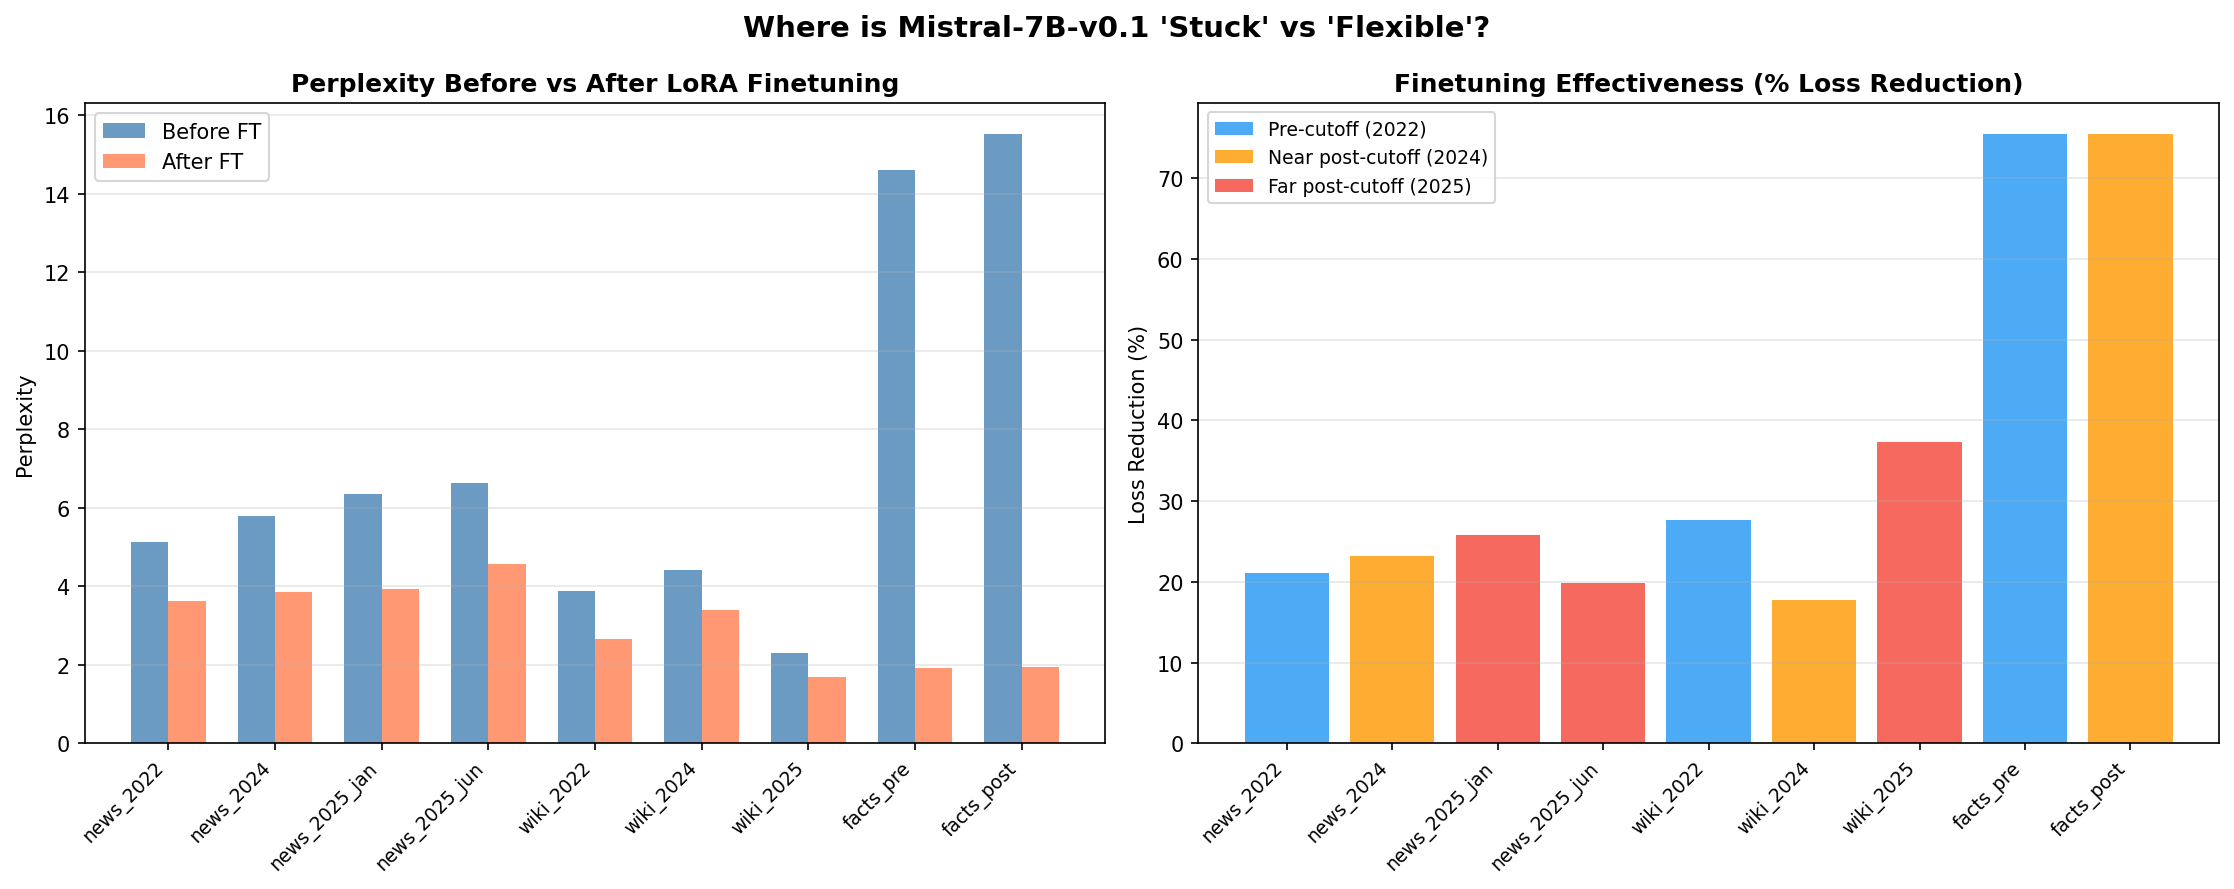
\includegraphics[width=0.95\linewidth]{figures/perplexity_comparison.png}
    \caption{Perplexity before (blue) and after (orange) fine-tuning across all conditions. News conditions show a persistent temporal gap even after fine-tuning, while factual QA conditions converge to near-identical final perplexity regardless of temporal distance. The pre/post gap for factual QA shrinks from 6.3\% to 1.2\% after training.}
    \label{fig:perplexity}
\end{figure}

\para{Factual QA text is highly learnable regardless of temporal distance.}
Despite the highest initial perplexity of any domain (14.61--15.54), factual QA text achieves the largest loss reduction (75.4--75.5\%). The pre/post-cutoff gap in initial perplexity is 6.3\%, but after fine-tuning this gap shrinks to 1.2\%---an 80\% gap closure. The convergence ratios (0.529 and 0.576) are also the lowest of any domain, indicating the strongest convergence. This reveals that the model efficiently learns the structured \emph{format} of the QA pairs (``As of [year], regarding [entity]: [question] The answer is: [answer]''), while the temporal content within that format has minimal impact on convergence.

\para{Wikipedia results are content-dependent, not time-dependent.}
The Wikipedia conditions show a non-monotonic pattern: \textsc{wiki-2025} actually has \emph{lower} initial perplexity (2.31) than \textsc{wiki-2022} (3.89). This inversion occurs because the specific articles in the 2025 condition happened to cover topics well-represented in the model's training data. With only 2--4 articles per condition, content specificity dominates over temporal effects. We discuss this limitation in \secref{sec:discussion}.

\subsection{Training Dynamics}

\Figref{fig:loss_curves} shows the training loss trajectories across conditions. News conditions exhibit a clear vertical offset---post-cutoff news trains from a higher initial loss---but all conditions follow similar descent patterns, suggesting that the learning \emph{rate} is consistent even when the learning \emph{target} is harder. Factual QA conditions show rapid initial descent followed by a long plateau, consistent with the model quickly learning the structural template and then slowly fitting individual examples.

\begin{figure}[t]
    \centering
    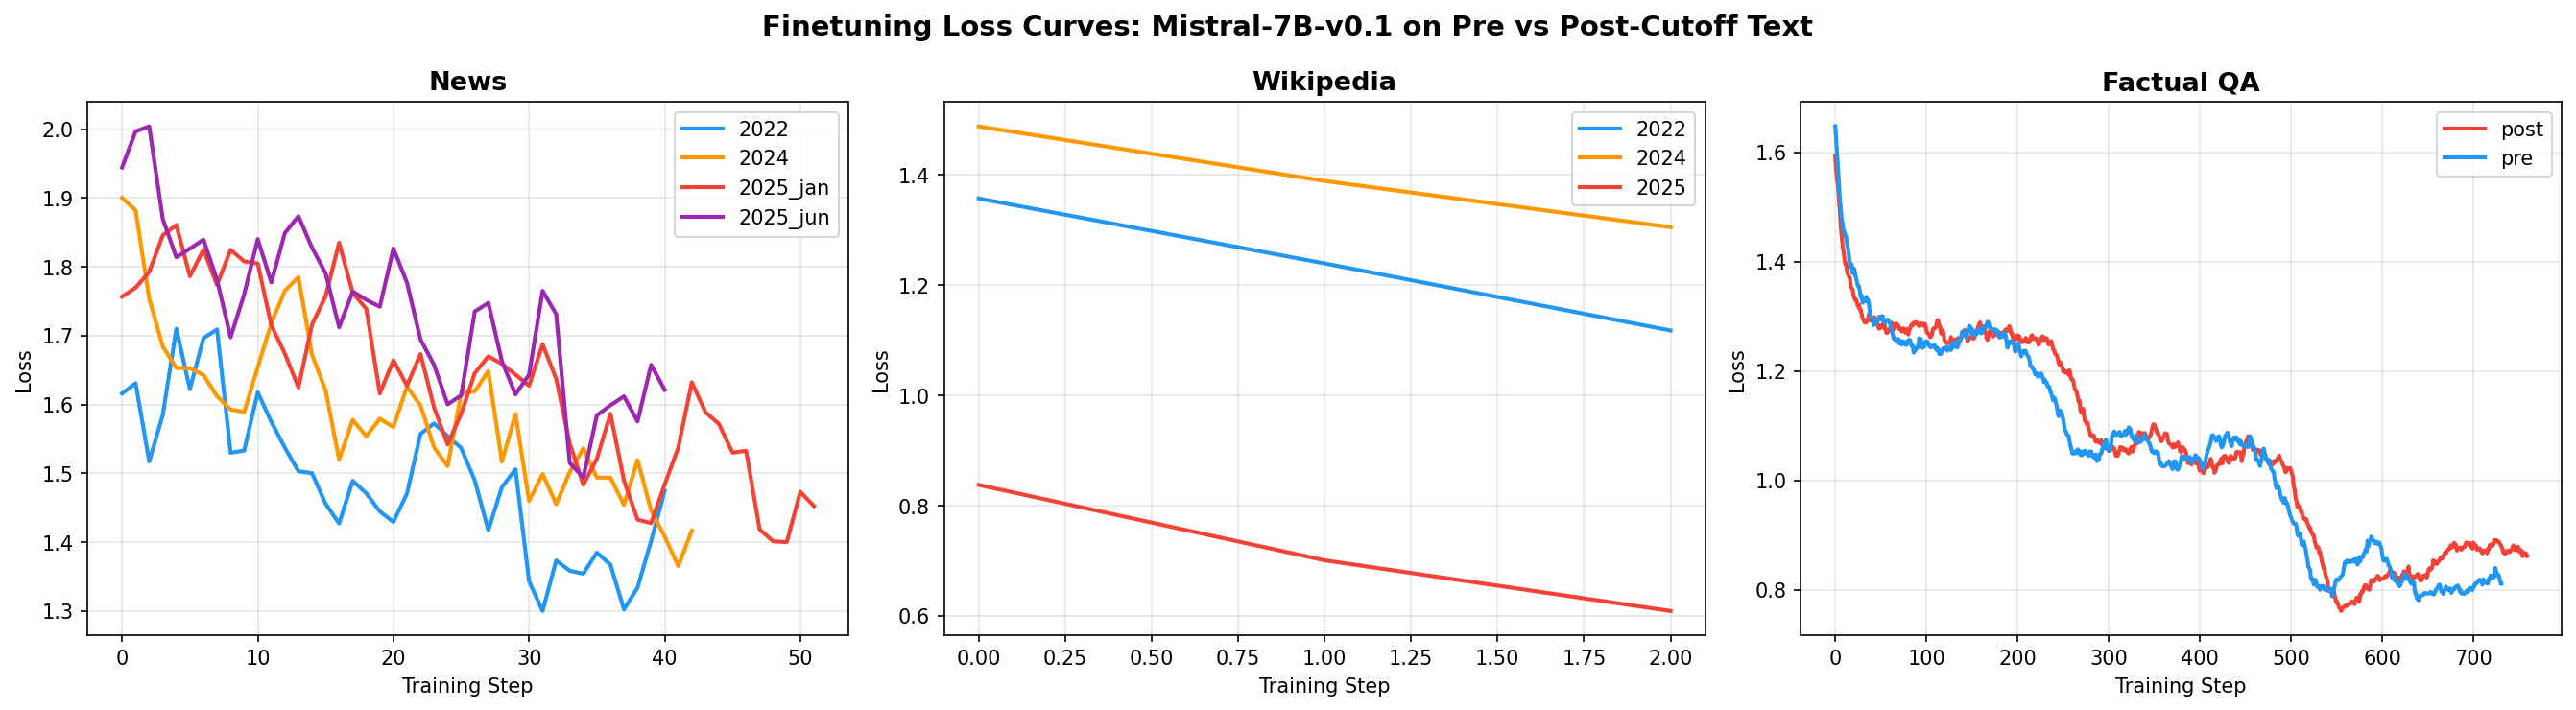
\includegraphics[width=0.95\linewidth]{figures/loss_curves_by_domain.png}
    \caption{Training loss curves by condition. News conditions (left group) show a persistent vertical offset proportional to temporal distance, while factual QA conditions (right group) converge to nearly identical final losses despite different starting points. The offset in news curves reflects irreducible uncertainty about novel entities and events.}
    \label{fig:loss_curves}
\end{figure}

\subsection{API Knowledge Probing Results}

\Tabref{tab:probing} presents the API probing results. \gptthree scores 4/30 correct (13.3\%) on post-cutoff questions, with all four correct answers involving events partially known before its cutoff: the Paris 2024 Olympics (announced pre-cutoff), OSIRIS-REx sample return (mission completed late 2023), Twitter/X rebrand (mid-2023), and Apple's \$3T market cap (trajectory established pre-cutoff).

\begin{table}[t]
    \centering
    \caption{API knowledge probing results by domain. Accuracy is the fraction of questions answered correctly. Both models predominantly \emph{decline} to answer (77--83\% of responses) rather than hallucinating, making it difficult to distinguish ``does not know'' from ``refuses to guess.''}
    \begin{tabular}{@{}lccc@{}}
        \toprule
        \textbf{Domain} & \textbf{\gptthree Acc.} & \textbf{\gptfourmini Acc.} & \textbf{Status} \\
        \midrule
        Politics & 0.00 & 0.00 & Stuck \\
        Technology & 0.00 & 0.10 & Stuck \\
        Entertainment & 0.00 & 0.20 & Stuck \\
        Science & 0.20 & 0.30 & Stuck \\
        Sports & 0.20 & 0.20 & Stuck \\
        Business & 0.40 & 0.20 & Moderate \\
        \midrule
        \textbf{Overall} & \textbf{0.133} & \textbf{0.167} & --- \\
        \bottomrule
    \end{tabular}
    \label{tab:probing}
\end{table}

\para{Knowledge type matters more than domain.}
Breaking down by knowledge type rather than domain, entity-specific knowledge (names, titles, specific outcomes) is hardest at 6\% accuracy, while pre-announced events achieve 29\% and ongoing trends 25\%. This aligns with the fine-tuning results: patterns and trajectories the model has partial knowledge of are accessible, while genuinely novel entities are not.

\subsection{Combined Analysis}

\Figref{fig:main} presents a combined view of all results. The key finding is consistent across both experiments: the boundary between ``stuck'' and ``flexible'' is not temporal distance per se, but whether the text requires \emph{novel factual knowledge} versus \emph{familiar structural patterns}. Fine-tuning is effective for the latter and ineffective for the former.

\begin{figure}[t]
    \centering
    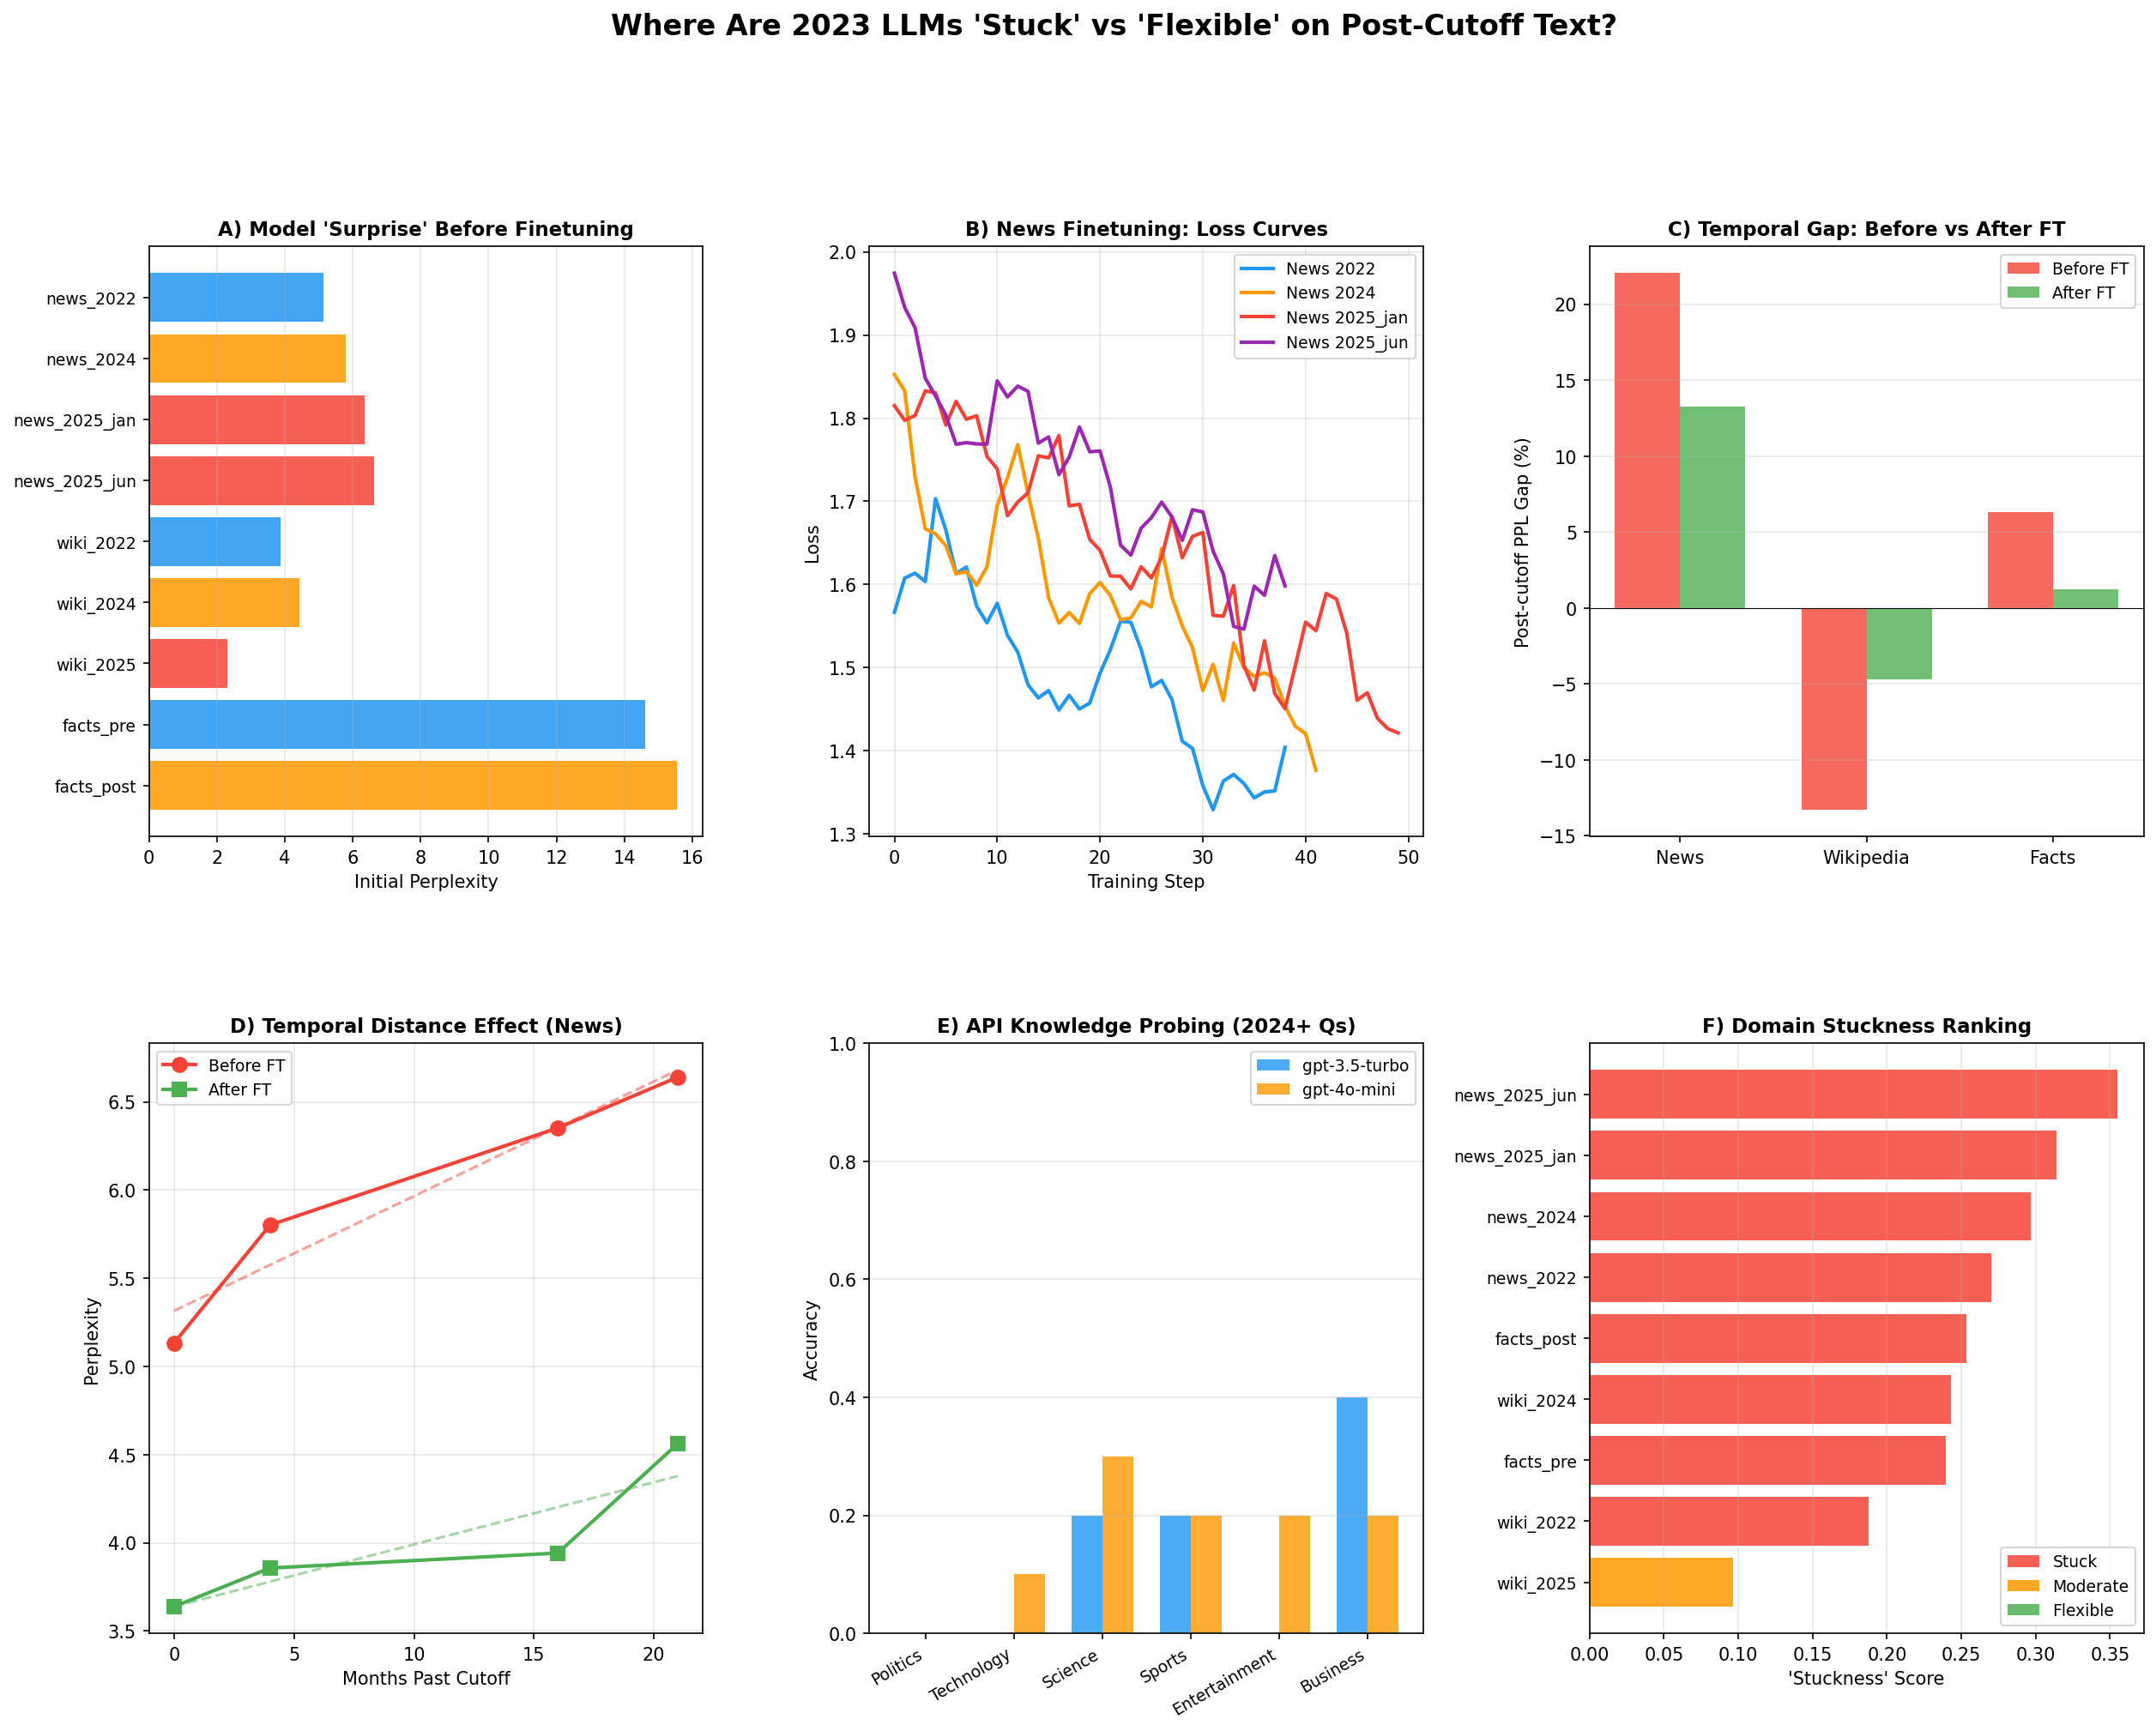
\includegraphics[width=0.95\linewidth]{figures/main_figure.png}
    \caption{Combined results across both experiments. \figtop: Fine-tuning convergence metrics by domain, showing that factual QA achieves high loss reduction regardless of temporal distance while news shows persistent gaps. \figbottom: API probing accuracy by domain and knowledge type, confirming that entity-specific knowledge is hardest to access post-cutoff.}
    \label{fig:main}
\end{figure}
